\documentclass[preview]{standalone}

\usepackage{amsmath}
\usepackage{amssymb}
\usepackage{stellar}
\usepackage{definitions}
\usepackage{bettelini}
\usepackage{tikz}

\begin{document}

\id{cantor-sets}
\genpage

\section{Cantor sets}

\begin{snippetdefinition}{cantor-set-definition}{Cantor set}
    \todo
\end{snippetdefinition}

\begin{snippet}{cantor-set-illustration}
    \begin{center}
    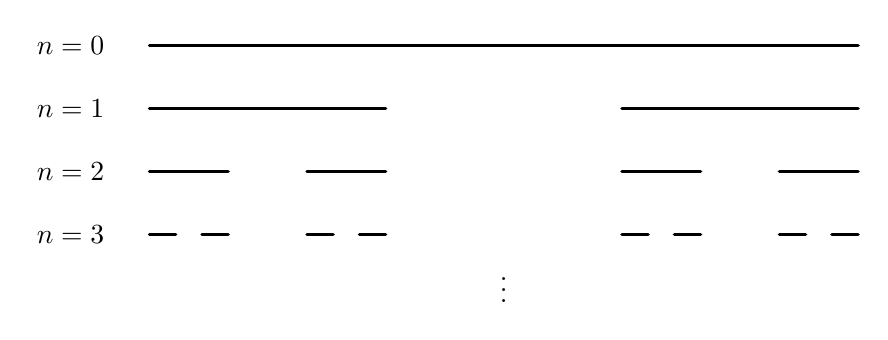
\begin{tikzpicture}[x=9cm,y=1cm,line cap=round]
        \foreach \y/\lbl in {0/0,-0.8/1,-1.6/2,-2.4/3}{
            \node[left] at (-0.05,\y) {$n=\lbl$};
        }

        \draw[line width=1.2pt] (0,0) -- (1,0);

        \draw[line width=1.2pt] (0,-0.8) -- (1/3,-0.8);
        \draw[line width=1.2pt] (2/3,-0.8) -- (1,-0.8);

        \foreach \a in {0,2/3}{
            \draw[line width=1.2pt] (\a,-1.6) -- ({\a+1/9},-1.6);
            \draw[line width=1.2pt] ({\a+2/9},-1.6) -- ({\a+1/3},-1.6);
        }

        \foreach \a in {0,2/9,2/3,8/9}{
            \draw[line width=1.2pt] (\a,-2.4) -- ({\a+1/27},-2.4);
            \draw[line width=1.2pt] ({\a+2/27},-2.4) -- ({\a+1/9},-2.4);
        }

        \node at (0.5,-3) {$\vdots$};
    \end{tikzpicture}
    \end{center}
\end{snippet}

\begin{snippetdefinition}{fat-cantor-set-definition}{Fat Cantor set}
    \todo
\end{snippetdefinition}

\end{document}